\chapter{Opis projektnog zadatka}
		
		
		\section{Potencijalna korist ovog projekta}

		U današnje doba, ljudima je ponekad teško pronaći druge sličnih interesa. KuhajIT je platforma upravo za pronalazak ljudi koji dijele interes za kuhanjem, nutricionizmom i ukusnom hranom. Cilj ovog projekta je razviti tu platformu i učiniti ju što lakšom za korištenje, kako bi kuharima entuzijastima te nutricionistima maksimalno uljepšali i pojednostavili korištenje platforme. Ono što bismo razvijanjem platforme KuhajIT dobili jest velika zajednica ljudi koji razmjenjuju iskustva, recepte, nova saznanja o nutritivnim vrijednostima, i sve im je to nadohvat ruke, udaljeno samo nekoliko klikova miša. Također, KuhajIT bi bila izvrsna platforma za one koji ne znaju kuhati ili žele usavršiti svoje vještine kuhanja, no ne znaju otkud početi.
		
		\section{Postojeća slična rješenja}
		
		Trenutno se u dubinama interneta nalazi nekolicina platformi koje djeluju po principu po kojem će djelovati platforma KuhajIT. Najsličnija platforma bila bi coolinarika. coolinarika je platforma koju je razvila Podravka za objavljivanje recepata od strane korisnika. Objavljene recepte ostali korisnici mogu recenzirati i ocjenjivati. To je ono po čemu su coolinarika i KuhajIT slične. Ono po čemu se coolinarika i KuhajIT razlikuju su različite vrste korisnika koje KuhajIT omogućava, dok coolinarika ne razlikuje svoje korisnike. Na taj način svatko tko se registrira može objaviti svoj recept, za razliku od KuhajIT platforme, gdje samo prijavljeni kulinarski entuzijasti mogu objavljivati svoje recepte, što platformi daje dodatni kredibilitet. Također, na platformi coolinarika ne postoji ni uloga 'nutricionista', koji na platformi KuhajIT slaže dijete i na taj način pomaže ostalim korisnicima. Platforma coolinarika ne nudi niti opciju skeniranja bar koda proizvoda za najbrži mogući dolazak do recepta koji je korisnik u danom trenutku u mogućnosti pripremiti.
		Druga slična platforma jest Index Recepti. Ta platforma također ne razlikuje svoje korisnike već svi imaju iste uloge. To znači da korisnik ne može raditi svoju kuharicu koja sadrži recepte, no može na stranicu dodati neki recept i na njega staviti određene tagove koji pomažu grupirati slične recepte različitih korisnika, što na KuhajIT nije omogućeno. Također, Index Recepti korisnicima daje mogućnost da njihovi recepti budu javni ili privatni, što znači da ih vidjeti mogu samo korisnici koji prime direktnu poveznicu na njih, dok na platformi KuhajIT svi korisnici mogu vidjeti sve recepte, tj. svi su recepti javni. Index Recepti, kao ni coolinarika, ne nudi opciju skeniranja bar koda proizvoda.
		
				\begin{figure}[H]
			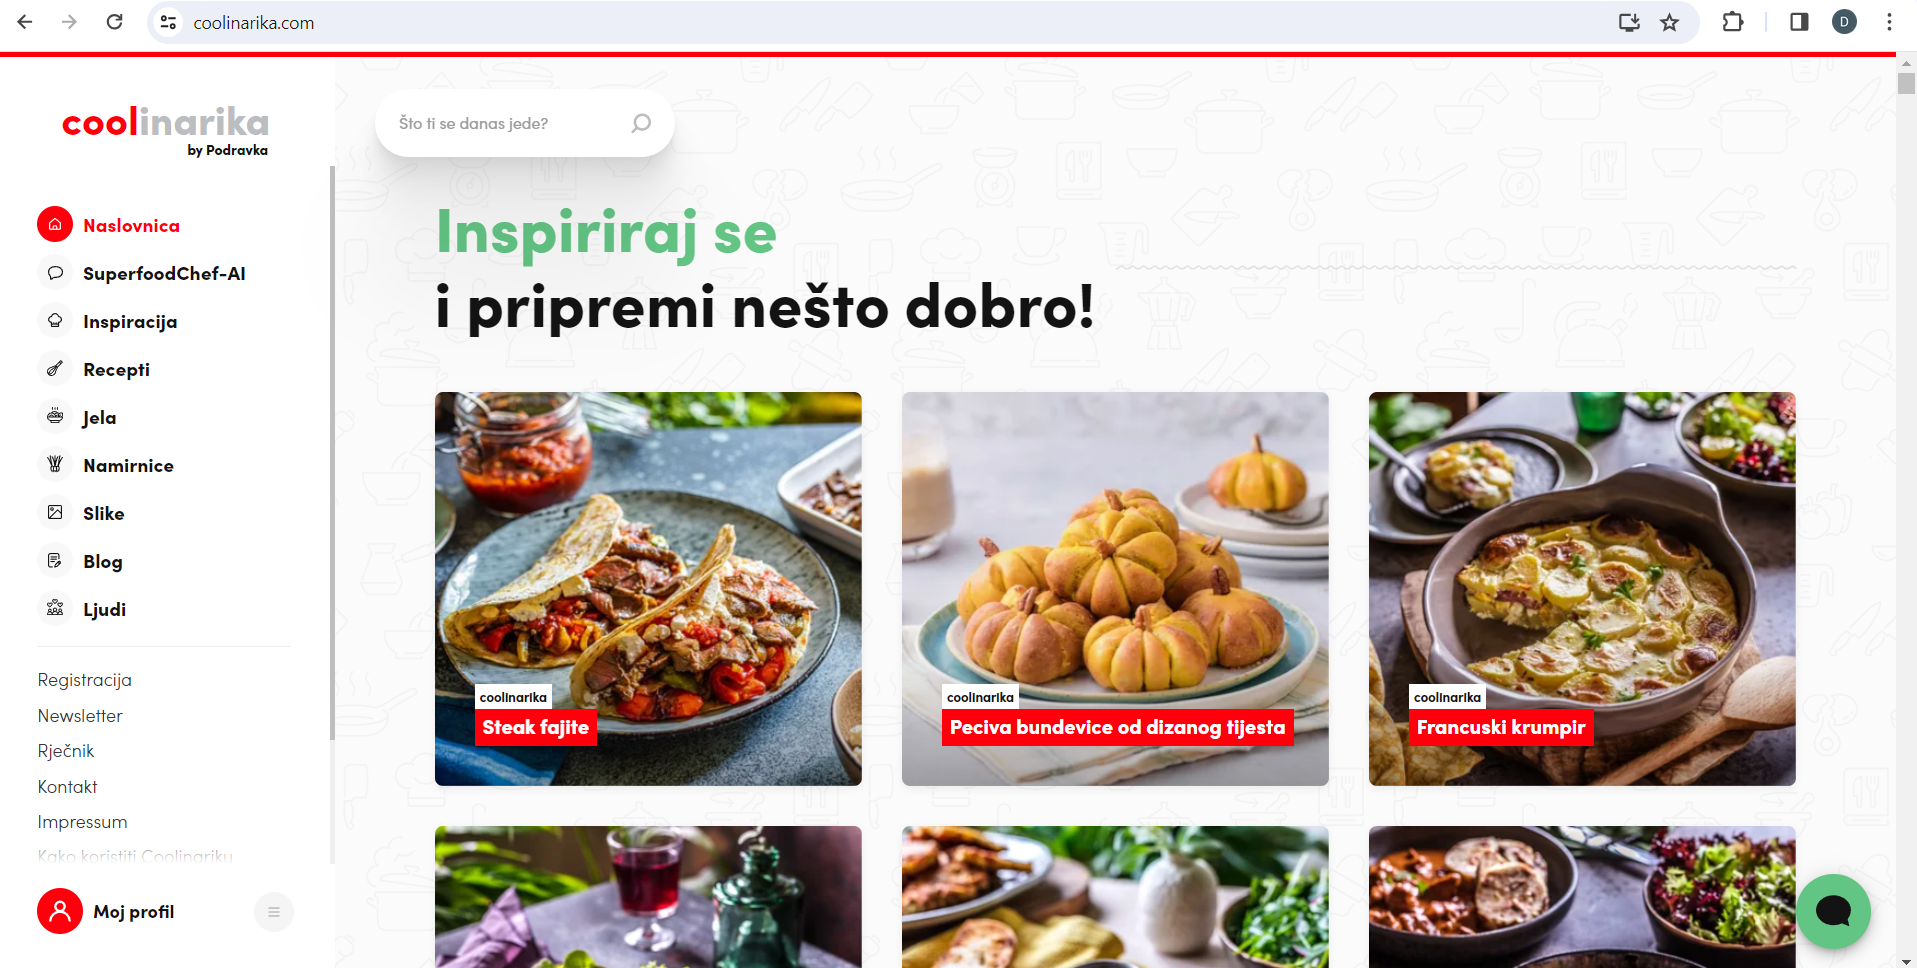
\includegraphics[scale=0.4]{slike/coolinarika.PNG} %veličina slike u odnosu na originalnu datoteku i pozicija slike
			\centering
			\caption{Sučelje platforme coolinarika}
			\label{coolinarika}
		\end{figure}
	
		\begin{figure}[H]
			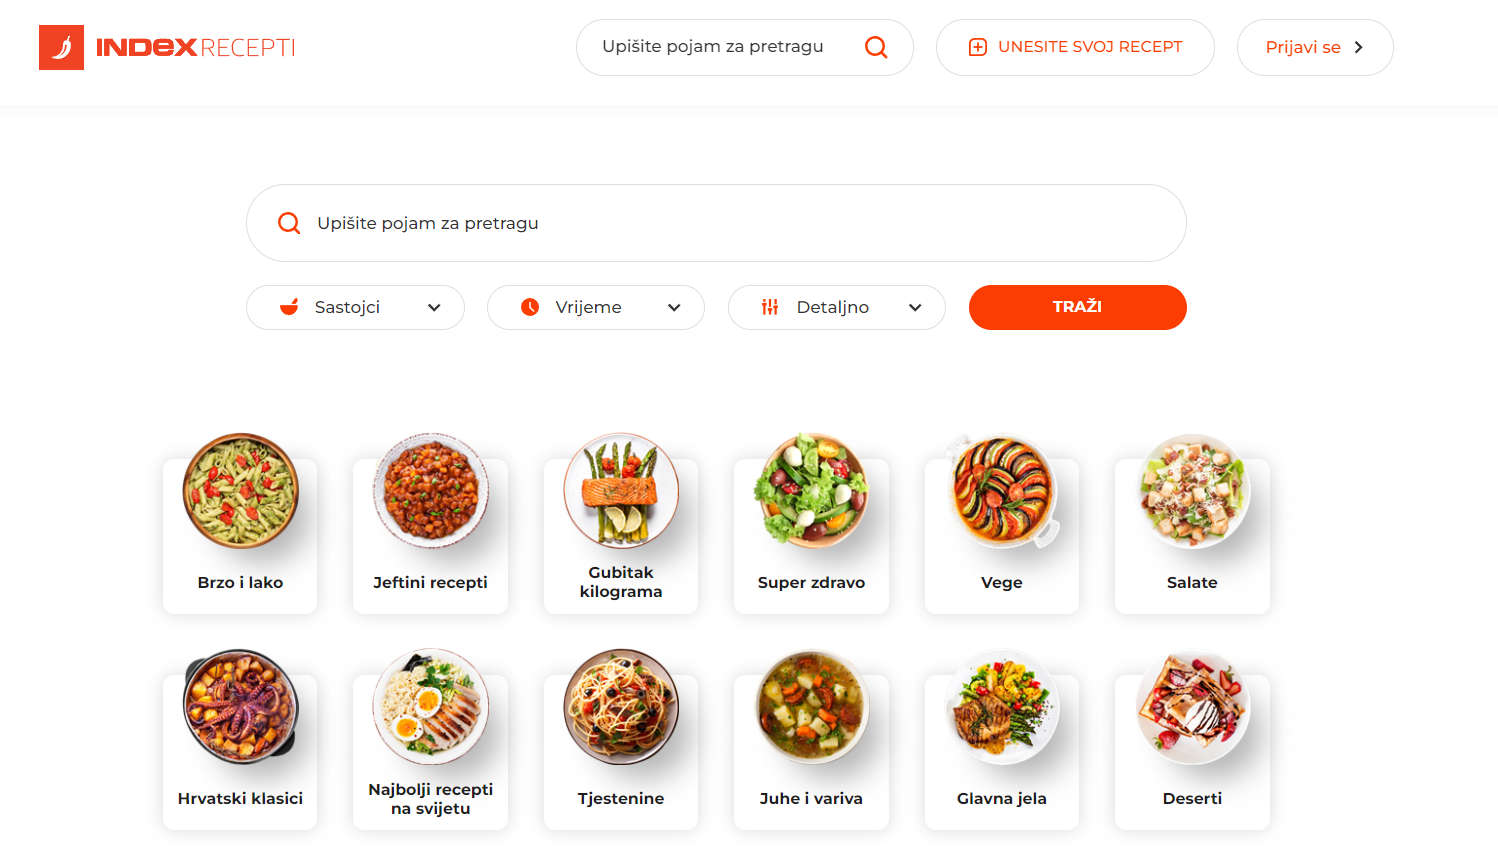
\includegraphics[scale=0.4]{slike/indexRecepti.PNG} %veličina slike u odnosu na originalnu datoteku i pozicija slike
			\centering
			\caption{Sučelje platforme Index Recepti}
			\label{indexRecepti}
		\end{figure}
		
		\section{Skup korisnika koji bi mogao biti zainteresiran za ostvareno rješenje}
		
		Za ovakvo rješenje mogli bi biti zainteresirani putni entuzijasti. Uz minimalne promjene platforme njezina tema bi se mogla promijeniti. Za temu putovanja promijenili bi recepte u mjesta koje bi ljudi mogli posjetiti. Tako bi umjesto sastojaka, uputstava i ostalih koraka vezanih za kuhanje, korisnici sada vidjeli znamenitosti određenog mjesta, parkove prirode ili nacionalne parkove u blizini i dodatne zanimljivosti koje bi bilo vrijedno pogledati. Kuharica bi sada bila regija ili država, a korisnici bi se dijelili na putopisce, kulturologe i avanturiste. Kulturolozi bi zamijenili kulinarske entuzijaste i mogli bi stvarati svoje "kuharice" tj. najbolja mjesta za posjetiti u određenoj regiji. Putopisci bi zamijenili nutricioniste, i umjesto "dijete" mogli bi korisnicima predložiti personaliziranu rutu ovisno o tome koje regije sve žele posijetiti i koji su njihovi interesi, odnosno u kojim dijelovima tih regija bi najviše mogli uživati. Klijenti bi ovdje bili avanturisti, ljudi koji žele putovati i na ovoj platformi traže ideje za mjesta vrijedna posjeta, kao i mogući putni vodič.
		
		\section{Opseg projektnog zadatka}
		Na platformi KuhajIT postoji opcija registracije.
		Neregistrirani korisnik može poslati zahtjev za registraciju u kojoj navodi i za koju se ulogu želi prijaviti. Moguće uloge su:
		\begin{packed_item}
		    \item klijent
		    \item kulinarski entuzijast
		    \item nutricionist
		\end{packed_item}
		
		Ako se neregistrirani korisnik želi prijaviti kao klijent, potrebno mu je sljedeće:
		\begin{packed_item}
			\item korisničko ime
			\item lozinka
			\item ime korisnika
			\item prezime korisnika
		\end{packed_item}
		
		Međutim, ako se neregistrirani korisnik želi prijaviti kao kulinarski entuzijast ili nutricionist, potrebno je još:
		\begin{packed_item}
			\item slika
			\item kratka biografija
			\item email
		\end{packed_item}
		
		Kako bi neregistrirani korisnik postao kulinarski entuzijast ili nutricionist na platformi KuhajIT, kao takvog ga mora potvrditi ADMINISTRATOR.
				Svi su registrirani korisnici, bili oni klijenti, kulinarski entuzijasti ili nutricionisti, u mogućnosti mijenjati podatke unutar svog KuhajIT profila. Neregistrirani korisnici nemaju tu mogućnost iz jednostavnog razloga što nisu registrirani, stoga ne posjeduju račun čije bi podatke mogli mijenjati.
	Svi korisnici, bili oni registrirani ili neregistrirani, mogu pretraživati i pregledavati recepte koje su objavili kulinarski entuzijasti. Na platformi postoji i mogućnost ostavljanja recenzija i ocjena na recepte i kuharice, koje mogu ostaviti svi korisnici, a autor recepta (kulinarski entuzijast koji je objavio recept) ima mogućnost odgovoriti na recenzije korisnika. Ako recenziju ostavi neregistrirani korisnik, on se vodi kao anoniman.
	Zadatak nutricionista je da unosi informacije o proizvodima (sastojcima jela), razvrstava ih u kategorije s oznakama te na temelju dostupnih informacijama o proizvodima izrađuje dijete za klijente i kulinarske entuzijaste platforme KuhajIT.
	Informacije o nutritivnim vrijednostima svakog proizvoda definirane su na 100g, a uključuju sljedeće:
	\begin{packed_item}
		\item energija
		\item masnoće
		\item zasićene masne kiseline
		\item ugljikohidrati
		\item šećeri
		\item bjelančevine
		\item sol
	\end{packed_item}
	
	Osim navedenog, svaki proizvod mora imati i priloženu fotografiju, masu i neke dodatke oznake koje ga svrstavaju u različite kategorije. Neke od dodatnih oznaka su:
		\begin{packed_item}
			\item "sadrži kikiriki"
			\item "sadrži gluten
			\item "riba"
			\item "tjestenina"
		\end{packed_item}
	
	Dijeta, koju nutricionist stvara, može se definirati s ograničenjima na određene proizvode, kategorije proizvoda, proizvode s nedopuštenim količinama sastojaka, te dnevnim limitom za određene nutritivne vrijednosti proizvoda. Dijeta sadrži i opis od nutricionista koji ju je stvorio.
	Kuharice su skupine recepata koje stvaraju kulinarski entuzijasti i nose tematski naziv, primjerice "Variva". Stvaranjem kuharice u njoj se ne nalazi niti jedan recept, a recepte u kuharice također dodaju njihovi autori, kulinarski entuzijasti. Međutim, to je opcionalno, odnosno ne mora svaki recept biti u pripadnoj kuharici, no isto tako, jedan recept može biti u više različitih kuharica istog kulinarskog entuzijasta. Tako se, primjerice, recept za varivo od graška može nalaziti u kuharici "Brzi ručkovi", a istovremeno i u kuharici "Priprema jela unaprijed". Valja napomenuti da je kulinarski entuzijast koji stvara kuharicu i sprema recepte u nju sam odgovoran za tematsku povezanost recepata u kuharici. Tako kulinarski entuzijast u kuharicu "Brzi ručkovi" teoretski može staviti i recept za čokoladnu tortu.
	Svaki recept je napisan po istom kalupu: najprije su navedeni svi potrebni sastojci, zajedno s njihovom količinom, i ukupno vrijeme kuhanja, zatim slijede koraci pripreme jela, popraćeni slikama koje pobliže objašnjavaju postupak. Naposljetku je navedena veličina jedne porcije jela uz popratnu sliku gotovog jela.
	Klijent platforme može skenirati bar kodove sastojaka, ili, ako neki od sastojaka nema bar kod, unijeti ga ručno iz dostupnih kategorija, koje ima doma i pomoću kojih želi pripremiti jelo, a na temelju tih sastojaka i ograničenja koje postavlja dijeta registriranog korisnika, platforma će pronaći i poredati recepte po njihovoj prihvatljivosti. Nakon što klijent odabere i pripremi odabrano jelo, on ga može označiti kao pripravljenog u tom danu, na temelju čega se, kroz dulji vremenski period, generira statistika konzumiranih nutritivnih vrijednosti u tom periodu.
	Neregistriranim se korisnicima prilikom otvaranja početne stranice prikazuju najnovije kuharice objavljene od strane kulinarskih entuzijasta. S druge strane,  registriranim korisnicima se na početnoj stranici prikazuju isprobani recepti, informacije o dijeti koju prate, nove kuharice i recepti od kulinarskih entuzijasta koje prate
	
		\section{Moguće nadogradnje projektnog zadatka}
		Neke od mogućih nadogradnji projektnog zadatka za platformu KuhajIT uključuju:
	\begin{packed_item}
		\item dodavanje video recepata
		\item chat u kojemu se registrirani korisnici mogu dopisivati s nutricionistima, kulinarskim entuzijastima i ostalima
		\item obavještavanje korisnika kada neki od kulinarskih entuzijasta koje prate objave novi recept ili kuharicu
		\item mogućnost ispisa željenog recepta
		\item "explore" dio na početnoj stranici registriranih korisnika, u kojem mogu otkriti neke nove kulinarske entuzijaste koji objavljuju recepte koji bi im se mogli svidjeti
		\item povezanost platforme s nekom internetskom trgovinom za kupnju namirnica, primjerice "Konzum Klik"
	\end{packed_item}
